\documentclass[tikz,border=4pt]{standalone}
\usepackage{amsmath}
\begin{document}
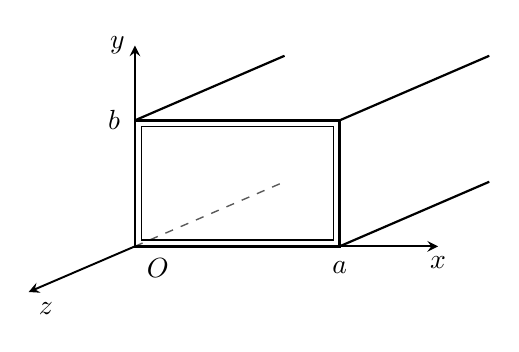
\begin{tikzpicture}[>=stealth, thick, scale=1.0]
  % Rectangular waveguide (z < 0 region shown, front face at z = 0)
  % O = (0,0), x goes right, y goes up, z goes down-left
  \def\aw{2.6}
  \def\bh{1.6}
  \coordinate (O) at (0, 0);
  \coordinate (Ax) at (\aw, 0);
  \coordinate (By) at (0, \bh);
  \coordinate (AB) at (\aw, \bh);
  \coordinate (Zneg) at (1.9, 0.82);

  % Hidden back edges inside waveguide
  \draw[dashed, line width=0.5pt, black!65] (O) -- ++(Zneg);

  % Outer top and right walls going to z < 0
  \draw[line width=0.8pt] (By) -- ++(Zneg);
  \draw[line width=0.8pt] (AB) -- ++(Zneg);
  \draw[line width=0.8pt] (Ax) -- ++(Zneg);

  % Front rectangular cross-section (double-wall look as in original)
  \draw[line width=0.9pt] (O) rectangle (AB);
  \draw[line width=0.4pt] (0.08, 0.08) rectangle ({\aw-0.08}, {\bh-0.08});

  % Axes
  \draw[->, line width=0.7pt] (Ax) -- (3.85, 0) node[below] {$x$};
  \draw[->, line width=0.7pt] (By) -- (0, 2.55) node[left] {$y$};
  \draw[->, line width=0.7pt] (O) -- (-1.35, -0.58) node[below right] {$z$};

  % Labels
  \node[below right] at (0.02, -0.02) {$O$};
  \node[below] at (\aw, -0.06) {$a$};
  \node[left] at (-0.06, \bh) {$b$};
\end{tikzpicture}
\end{document}
